\documentclass[12pt,a4paper]{report}
\usepackage[french]{babel}
\usepackage{graphicx}
\usepackage{hyperref}
\usepackage{float}
\usepackage{url}
\usepackage{enumitem}
\usepackage[T1]{fontenc}
\usepackage[utf8]{inputenc}
\usepackage{csquotes}
\usepackage{geometry}
\usepackage{titlesec}
\usepackage{fancyhdr}
\usepackage{xcolor}
\usepackage{tikz}
\usepackage{tcolorbox}

% Configuration de la géométrie de la page
\geometry{
	top=2.5cm,
	bottom=2.5cm,
	left=2.5cm,
	right=2.5cm
}

% Configuration des titres
\titleformat{\chapter}[display]
{\normalfont\huge\bfseries}{\chaptertitlename\ \thechapter}{20pt}{\Huge}
\titlespacing*{\chapter}{0pt}{-50pt}{40pt}

% Configuration des en-têtes et pieds de page
\pagestyle{fancy}
\fancyhf{}
\renewcommand{\headrulewidth}{0.4pt}
\fancyhead[L]{\leftmark}
\fancyhead[R]{\thepage}

% Création de la page de garde
\begin{document}
	
	% Suppression des numéros de page sur la page de garde
	\pagenumbering{gobble}
	
	\begin{titlepage}
		\begin{center}
			
			% Logo de l'université (à remplacer par votre logo)
			\vspace*{-1cm}
			\begin{figure}[h]
				\centering
				
\includegraphics[width=0.4\textwidth]{images/logo_university.png}
			\end{figure}
			
			\vspace{1cm}
			
			{\LARGE\textbf{Université Sidi Mohamed Ben Abdellah De Fes}}\\[0.5cm]
			{\Large Faculé de science}\\[0.5cm]
			{\large Web Intelligence Et Sciences De Données (WISD)}
			
			\vspace{2cm}
			
			\begin{tcolorbox}[colback=gray!5,colframe=gray!40,width=\textwidth,arc=0mm]
				\begin{center}
					{\Huge\textbf{Rapport de Projet}}\\[0.5cm]
					{\LARGE\textbf{Application Mobile Marketplace}}\\[0.3cm]
					{\huge\textcolor{gray}{\textbf{« SwapChic »}}}
				\end{center}
			\end{tcolorbox}
			
			\vspace{2cm}
			
			\begin{minipage}{0.4\textwidth}
				\begin{flushleft}
					\large\textbf{Réalisé par :}\\
					Salma LAKEHAL\\
					Abdelilah EL GALLATI
				\end{flushleft}
			\end{minipage}
			\hfill
			\begin{minipage}{0.4\textwidth}
				\begin{flushright}
					\large\textbf{Encadré par :}\\
					Mr. Khalid EL FAHSSI
				\end{flushright}
			\end{minipage}
			
			\vfill
			
			{\large Année Universitaire : 2024/2025}
			
		\end{center}
	\end{titlepage}
	
	\pagenumbering{roman}

	\newpage
	\newpage
	
	\chapter*{Remerciements}
	Nous souhaitons remercier chaleureusement notre professeur \textbf{Mr. El Fahssi Khalid} pour son accompagnement tout au long de ce projet. Ses conseils avisés, sa bienveillance et sa disponibilité ont été une source d'encouragement et d'inspiration pour nous.
	
	Grâce à son soutien, nous avons pu non seulement progresser dans le développement de notre application, mais aussi apprendre de nouvelles méthodes et renforcer nos compétences. Son approche pédagogique, toujours à l'écoute, nous a permis de mieux comprendre nos erreurs et de trouver des solutions adaptées.
	
	Nous gardons une grande reconnaissance pour tout le temps et l'énergie qu'il a consacrée à nous guider. Ce projet n'aurait pas été le même sans sa précieuse aide.
	
	\chapter*{Résumé}
	SwapChic est une application dédiée à l'échange de produits entre utilisateurs. Elle permet à chaque utilisateur de créer un compte, gérer son profil, publier des annonces de produits qu'il souhaite échanger, et rechercher des articles disponibles. Grâce à une interface de messagerie, les utilisateurs peuvent entrer en contact, proposer des échanges, et finaliser des transactions. Un administrateur veille à la gestion des utilisateurs et à la modération des annonces.
	
	Cette application vise à offrir une solution pratique pour le troc de produits, en facilitant l'accès à un large catalogue d'articles tout en garantissant la sécurité et la transparence des échanges. SwapChic se positionne comme une plateforme éthique favorisant la consommation responsable.
	
	\tableofcontents
	\newpage
	\listoffigures
	\newpage
	\listoftables
	\newpage
	
	
	\chapter{Introduction Générale}
	\newpage
	\section{Introduction}
	Dans un monde où la consommation évolue rapidement et où la prise de conscience écologique gagne du terrain, les modes de vie changent pour adopter des solutions plus durables et responsables. Cependant, l'échange d'objets de seconde main reste souvent limité par des barrières logistiques, de confiance ou d'accessibilité. Face à ces défis, notre projet \textbf{SwapChic} se positionne comme une réponse innovante, visant à révolutionner la manière dont les individus échangent des produits de seconde main.
	
	Ce projet s'inscrit dans une vision ambitieuse : concevoir et développer une application mobile intuitive et performante qui simplifie les échanges entre particuliers. Notre objectif principal est d'offrir une plateforme conviviale permettant aux utilisateurs de donner une seconde vie à leurs objets tout en favorisant un mode de consommation éthique et éco-responsable.
	
	Au centre de notre réflexion, une problématique essentielle : comment créer une application mobile qui allie simplicité d'utilisation, sécurité des échanges, et valorisation des produits tout en promouvant les principes d'économie circulaire ? Cette question constitue le fil conducteur de notre démarche dans ce projet.
	
	À travers ce rapport, nous présenterons les objectifs de notre application, les défis auxquels nous devrons faire face, ainsi que les fonctionnalités clés qui garantiront une expérience utilisateur optimale. Animés par la volonté d'encourager un mode de consommation durable et de rapprocher les utilisateurs, nous sommes engagés à transformer les obstacles en opportunités, et à faire de \textbf{SwapChic} un outil incontournable pour la communauté.
	
	\section{Contexte de Projet}
	Les avancées technologiques ont révolutionné de nombreux aspects de nos vies, mais le domaine de l'économie circulaire et de l'échange d'objets de seconde main reste encore en attente de solutions pratiques et accessibles. Les limitations en termes de simplicité, de confiance et d'efficacité dans les échanges peuvent souvent décourager les utilisateurs. C'est dans ce contexte que s'inscrit notre projet \textbf{SwapChic}, avec pour ambition d'améliorer considérablement les interactions et les échanges de produits entre particuliers, tout en adoptant une démarche éco-responsable et durable.
	
	\section{Cahier de Charge}
	\subsection{Objectif}
	Le projet \textbf{SwapChic} a pour objectif de développer une application mobile innovante qui facilite les échanges de produits d'occasion entre particuliers. Elle permet aux utilisateurs de vendre, acheter, donner, prêter ou échanger temporairement des articles tout en promouvant une culture de réutilisation responsable. L'application aspire à réduire le gaspillage, encourager une économie circulaire, et rendre ces pratiques accessibles, sécurisées et intuitives pour tous.
	
	\subsection{Problématique}
	Comment concevoir une application mobile qui simplifie et sécurise les échanges de produits d'occasion tout en garantissant une expérience utilisateur fluide ? L'objectif est également de surmonter des défis tels que la confiance entre utilisateurs, la gestion des transactions, et la création d'une plateforme intuitive qui encourage l'adoption massive de pratiques éco-responsables.
	
	\subsection{Fonctionnalités principales}
	\subsubsection{Gestion des utilisateurs}
	\begin{itemize}
		\item Inscription via e-mail ou réseaux sociaux.
		\item Création de profils personnalisés avec nom, photo, localisation, et historique d'activités.
	\end{itemize}
	
	\subsubsection{Catalogue de produits}
	\begin{itemize}
		\item Classement des produits par catégories (livres, vêtements, jouets, etc.).
		\item Recherche avancée avec filtres (localisation, prix, catégorie, état du produit).
		\item Possibilité d'ajouter des produits avec photos, description, prix (si applicable) et conditions d'échange ou de prêt.
	\end{itemize}
	
	\subsubsection{Interaction entre utilisateurs}
	\begin{itemize}
		\item Système de messagerie intégré pour négociations.
		\item Système de commentaires et d'évaluations pour noter les produits et les utilisateurs.
	\end{itemize}
	
	\subsubsection{Gestion des échanges}
	\begin{itemize}
		\item Notifications automatiques pour rappeler les échéances de retour en cas de prêt.
		\item Suivi des transactions dans un tableau de bord utilisateur.
	\end{itemize}
	
	
	\chapter{Conception et Planification}
	
	\newpage
	
	\section{Introduction}
	Le chapitre de conception et planification constitue une étape essentielle dans le processus de développement de notre application de communication dédiée à la santé. Dans ce chapitre, nous aborderons en détail la planification du projet, qui inclut le diagramme de tâches, le diagramme de modèle en V, ainsi que le diagramme de Gantt. Ensuite, nous nous concentrerons sur la conception proprement dite de l'application, en décrivant les cas d'utilisation, le diagramme de classes, et le diagramme de séquence.
	
	\section{Planification}
	\subsection{Découpage du projet en tâches}
	Le découpage du projet en tâches consiste à diviser le travail en différentes activités ou étapes gérables et distinctes. Cela permet une meilleure organisation, une répartition efficace des responsabilités et une planification précise des activités à réaliser pour atteindre les objectifs du projet.
	
	\begin{figure}[H]
		\centering
		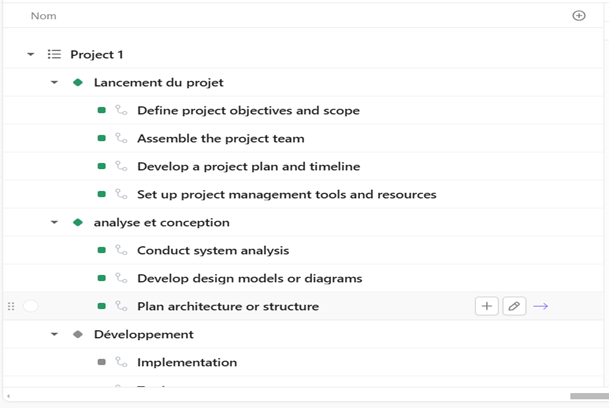
\includegraphics[width=0.8\textwidth]{images/taches_projet.png}
		\caption{Découpage du projet en tâches}
		\label{fig:decoupage}
	\end{figure}
	
	\subsection{Cycle de vie en modèle V}
	Le cycle de vie en modèle V définit parallèlement les démarches afférentes à mettre en place en termes d'assurance qualité et détaille la façon dont les différentes phases doivent interagir entre elles.
	
	\begin{figure}[H]
		\centering
		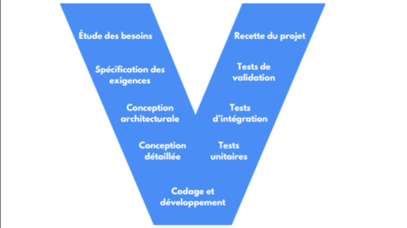
\includegraphics[width=0.6\textwidth]{images/cycle_vie.png}
		\caption{Cycle de vie en modèle V}
		\label{fig:cycle_v}
	\end{figure}
	
	\subsection{Diagramme de Gantt}
	Le diagramme de Gantt est l'un des outils les plus efficaces pour décrire les phases d'un projet et une représentation claire de l'état de l'avancement de ses différentes tâches.
	
	\begin{figure}[H]
		\centering
		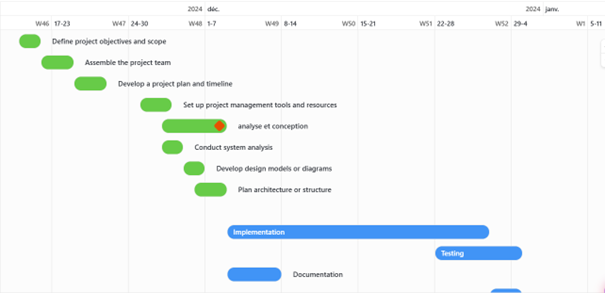
\includegraphics[width=0.8\textwidth]{images/diagramme_gant.png}
		\caption{Diagramme de Gantt}
		\label{fig:gantt}
	\end{figure}
	
	\section{Modélisation en UML}
	\subsection{Présentation du langage UML}
	Le langage de modélisation unifié (UML) est un langage général, de développement, de modélisation dans le domaine de l'ingénierie logicielle qui est destiné à fournir un moyen standard de visualiser la conception d'un système.
	
	\subsection{Cas d'utilisation}
	\subsubsection{Définition}
	Les diagrammes de cas d'utilisation (DCU) sont des diagrammes UML utilisés pour une représentation du comportement fonctionnel d'un système logiciel.
	
	\subsubsection{Cas d'utilisation de l'application web}
	Pour respecter le cahier de charge, les éléments constituant du DCU de l'application sont décrits comme suit :
	
	\begin{itemize}
		\item \textbf{Patient}
		\begin{itemize}
			\item Créer un compte
			\item Se connecter
			\item Mettre à jour son profil
			\item Ajouter un produit
			\item Rechercher des produits
			\item Recevoir des notifications
			\item Gérer ses transactions
			\item Échanger / Vendre / Donner un produit
			\item Noter un produit ou un utilisateur
			\item Contacter un autre utilisateur
		\end{itemize}
		\item \textbf{Administrateur}
		\begin{itemize}
			\item Modérer les contenus
			\item Vérifier les identités
			\item Gérer les utilisateurs
		\end{itemize}
	\end{itemize}
	
	\begin{figure}[H]
		\centering
		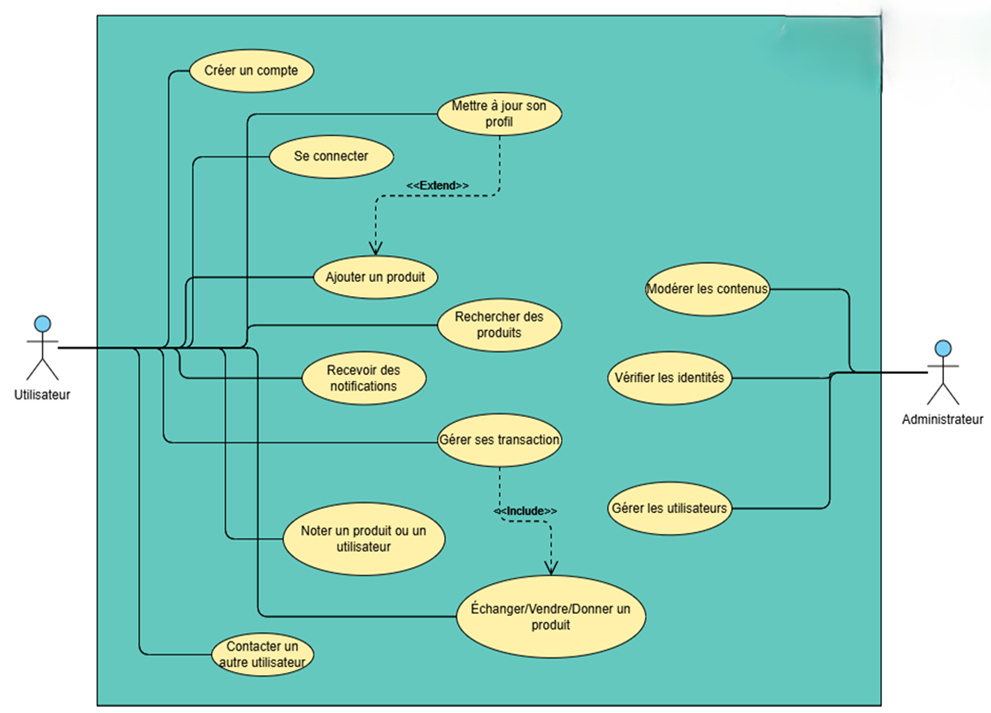
\includegraphics[width=0.8\textwidth]{images/use_case.png}
		\caption{Diagramme de cas d'utilisation}
		\label{fig:cas_utilisation}
	\end{figure}
	
	\subsection{Diagramme de classes}
	\subsubsection{Définition}
	Le diagramme de classes est un schéma utilisé en génie logiciel pour présenter les classes et les interfaces des systèmes ainsi que leurs relations.
	
	\subsubsection{Diagramme de classe de notre application web}
	Pour la modélisation de notre diagramme de classes, nous avons opté pour les sept classes suivantes : User, Product, Message, Transaction, Category, Notification, Review.
	
	\begin{figure}[H]
		\centering
		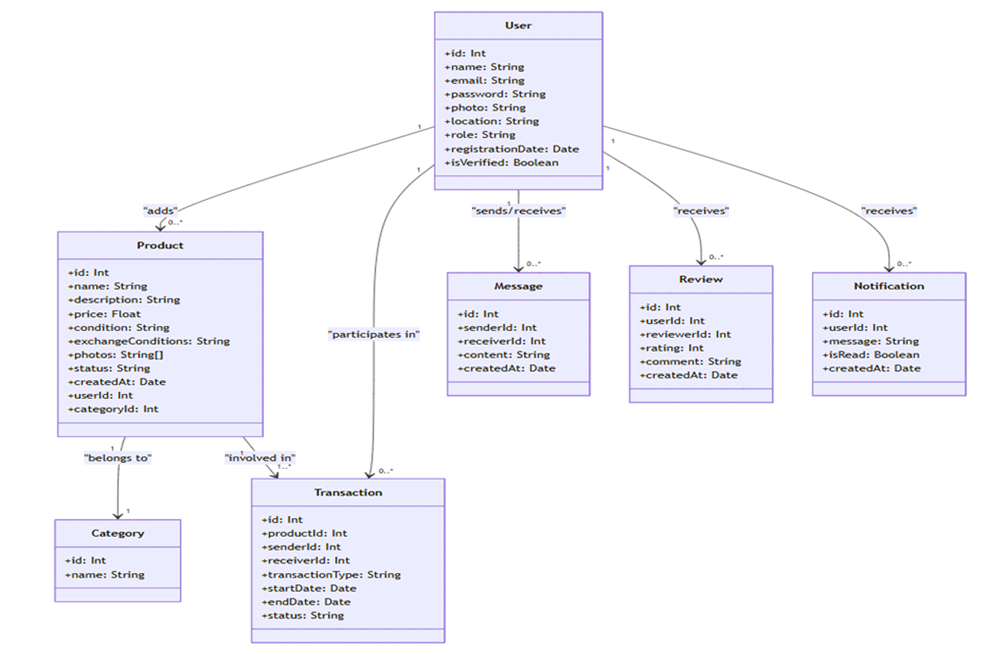
\includegraphics[width=0.8\textwidth]{images/class_diagram.png}
		\caption{Diagramme de classes}
		\label{fig:diagramme_classes}
	\end{figure}
	
	\subsection{Diagramme de séquence}
	\subsubsection{Définition}
	Les diagrammes de séquences modélisent la représentation graphique des interactions entre les acteurs et le système, selon un ordre chronologique dans la formulation UML.
	
	\subsubsection{Scénario : Connexion des utilisateurs}
	Le diagramme de séquence présenté illustre un scénario modélisant le processus d'authentification d'un utilisateur dans un système en ligne.
	
	\begin{figure}[H]
		\centering
		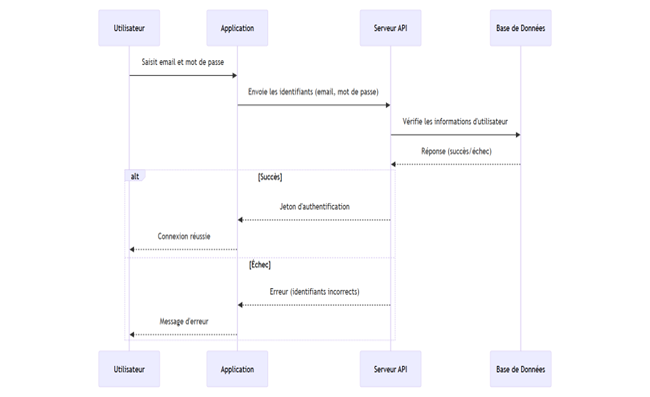
\includegraphics[width=0.8\textwidth]{images/authentification_scenario.png}
		\caption{Diagramme de séquence : Connexion des utilisateurs}
		\label{fig:sequence_connexion}
	\end{figure}
	
	\subsubsection{Scénario : Recherche des articles}
	Ce diagramme de séquence représente le processus de recherche de produits dans une application.
	
	\begin{figure}[H]
		\centering
		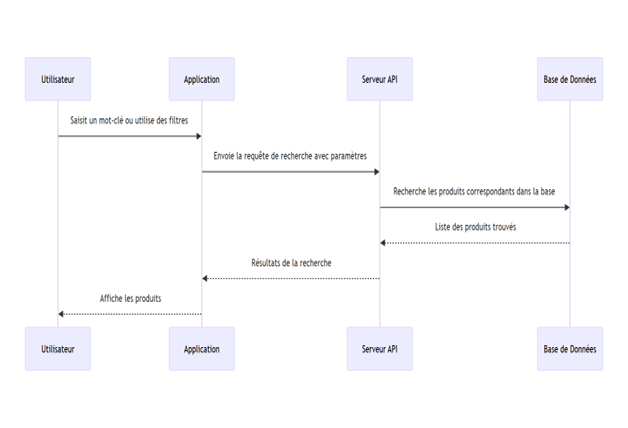
\includegraphics[width=0.8\textwidth]{images/recherche_scenario.png}
		\caption{Diagramme de séquence : Recherche des articles}
		\label{fig:sequence_recherche}
	\end{figure}
	
	\subsubsection{Scénario : Transaction}
	Le diagramme de séquence présenté montre le processus d'une demande entre un demandeur et un offreur.
	
	\begin{figure}[H]
		\centering
		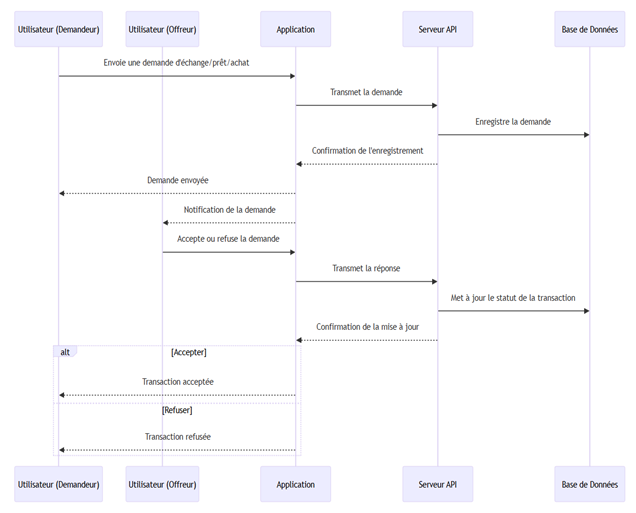
\includegraphics[width=0.8\textwidth]{images/transaction_scenario.png}
		\caption{Diagramme de séquence : Transaction}
		\label{fig:sequence_transaction}
	\end{figure}
	
	\section{Conclusion}
	Ce chapitre a offert une vision globale de notre travail en présentant l'aspect analytique et conceptuel de l'application \textbf{SwapChic} à travers les diagrammes UML. Nous avons détaillé les différentes classes et leurs associations, ce qui a permis de structurer les relations essentielles pour le bon fonctionnement du système d'échange de produits. Grâce à cette modélisation, nous avons clarifié les interactions entre les utilisateurs (demandeurs et offreurs) ainsi que les éléments clés comme les demandes d'échange, les notifications et les mises à jour des transactions.
	
	Le chapitre suivant sera consacré à la mise en œuvre et à la réalisation de notre application, où nous aborderons les aspects techniques et pratiques de son développement, en explorant les défis rencontrés et les solutions mises en place pour garantir une expérience utilisateur fluide et efficace.
	
	\chapter{Mise en Œuvre et Réalisation}
	
	\newpage
	
	\section{Introduction}
	La phase de réalisation est l'aboutissement des phases précédentes, car c'est dans celle-ci que le produit du projet, pensé et décrit dans la phase de définition, est concrétisé. Nous présentons dans ce chapitre les différentes étapes de la réalisation de notre application web. Nous commençons en premier lieu par l'environnement de travail et les outils de développement utilisés. En second lieu, nous passons à la transformation des classes UML en modèle logique et à la création de la base de données ainsi que l'implémentation du modèle MVC. Et finalement, nous élaborons une présentation des différentes interfaces développées.
	
	\section{Outils et Technologies Utilisés}
	

	
	\subsection{Environnement de Développement}
	\begin{figure}[H]
		\centering
		\begin{tabular}{cccc}
			
\includegraphics[width=0.15\textwidth]{images/vs_code.jpg} &
			
\includegraphics[width=0.15\textwidth]{images/visual_paradigm.png} &
			
\includegraphics[width=0.15\textwidth]{images/clickup.png} &
			
\includegraphics[width=0.15\textwidth]{images/mermaid_live_editor.png} \\
			\textbf{Visual Studio Code} & \textbf{Visual Paradigm} & \textbf{ClickUp} & \textbf{Mermaid Live} \\
			Éditeur de code & Modélisation UML & Gestion de projet & Création de diagrammes \\
		\end{tabular}
		\caption{Outils de développement et de gestion de projet}
	\end{figure}
	
	\subsection{Stack Technique}
	\begin{figure}[H]
		\centering
		\begin{tabular}{ccc}
			
\includegraphics[width=0.15\textwidth]{images/react_native.png} &
			
\includegraphics[width=0.15\textwidth]{images/mongodb.png} &
			
\includegraphics[width=0.15\textwidth]{images/nodejs.png} \\
			\textbf{React Native} & \textbf{MongoDB} & \textbf{Node.js} \\
			Frontend mobile & Base de données & Backend \\
		\end{tabular}
		\caption{Technologies principales du projet}
	\end{figure}
	

	
	
	\section{Fonctionnalités principales}
	La section suivante est dédiée à la présentation de l'application que nous avons développée. Nous avons choisi d'utiliser des exemples clairs pour illustrer chaque cas d'utilisation de notre interface de manière efficace.
	
	\subsection{Gestion des utilisateurs}
	\begin{itemize}
		\item \textbf{Inscription via Google} : Permet aux utilisateurs de s'inscrire rapidement en utilisant leur compte Google.
	\end{itemize}
	
	\subsection{Catalogue de produits}
	\begin{itemize}
		\item \textbf{Classement des produits par catégories} : Les produits sont organisés en catégories telles que :
		\begin{itemize}
			\item Livres
			\item Vêtements
			\item Jouets
			\item Appareils ménagers
			\item etc.
		\end{itemize}
		\item \textbf{Recherche avancée avec filtres} : Les utilisateurs peuvent filtrer les produits par :
		\begin{itemize}
			\item Nom du produit
			\item Catégorie
		\end{itemize}
		\item \textbf{Ajout de produits par les utilisateurs} : Les utilisateurs peuvent ajouter des produits en fournissant :
		\begin{itemize}
			\item Des photos
			\item Une description détaillée
			\item Un prix (si applicable)
			\item Les conditions d'échange ou de prêt
		\end{itemize}
	\end{itemize}
	
	\subsection{Interaction entre utilisateurs}
	\begin{itemize}
		\item \textbf{Messagerie intégrée} : Un système de messagerie permet aux utilisateurs de négocier et de discuter des détails des transactions.
		\item \textbf{Système de likes} : Les utilisateurs peuvent noter les produits et les autres utilisateurs en utilisant un système de likes.
	\end{itemize}
	
	\subsection{Échange et gestion des produits}
	\begin{itemize}
		\item \textbf{Suivi des transactions} : Les utilisateurs peuvent suivre l'état de leurs transactions via un tableau de bord personnalisé.
	\end{itemize}
	
	\section{Réalisation}
	Cette section présente les principales interfaces de l'application \textbf{SwapChic}, développée dans le cadre du projet. Chaque capture d'écran est accompagnée d'une description détaillée pour expliquer les fonctionnalités et les éléments clés de l'interface.
	
	\subsection{Page d'accueil}
	\begin{figure}[H]
		\centering
		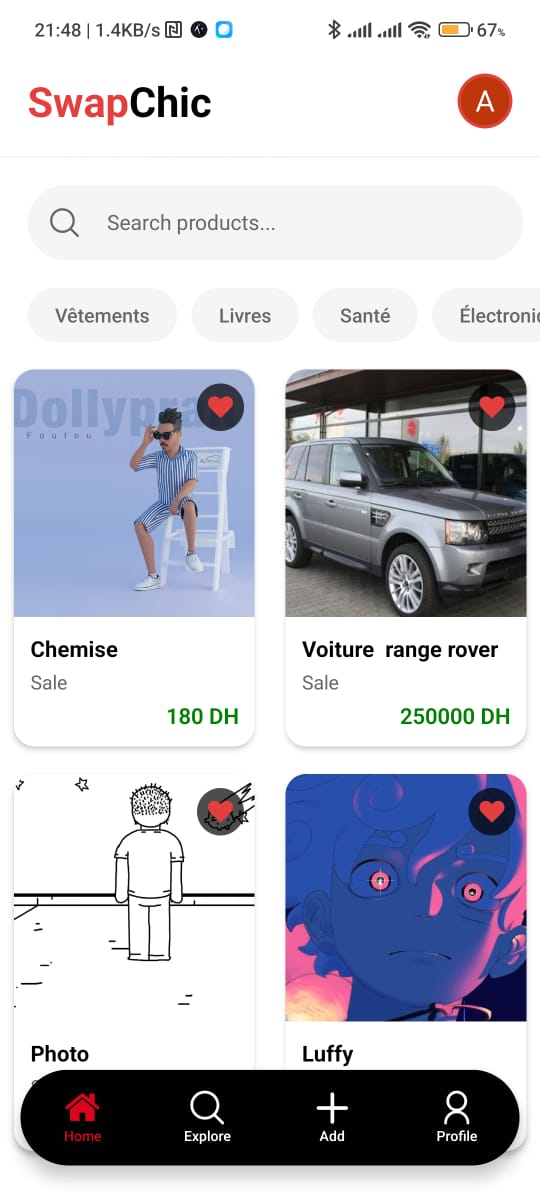
\includegraphics[width=0.8\textwidth]{images/home_page.png} % Remplacez par le chemin de votre capture d'écran
		\caption{Page d'accueil de l'application SwapChic. Cette interface présente les produits récents et les catégories populaires, permettant aux utilisateurs de naviguer facilement.}
		\label{fig:home_page}
	\end{figure}
	
	\subsection{Page d'inscription}
	\begin{figure}[H]
		\centering
		\includegraphics[width=0.8\textwidth]{images/signup_page.png} % Remplacez par le chemin de votre capture d'écran
		\caption{Page d'inscription de l'application. Les utilisateurs peuvent s'inscrire via Google ou en remplissant un formulaire manuel.}
		\label{fig:signup_page}
	\end{figure}
	
	\subsection{Catalogue de produits}
	\begin{figure}[H]
		\centering
		\includegraphics[width=0.8\textwidth]{images/product_catalog.png} % Remplacez par le chemin de votre capture d'écran
		\caption{Catalogue de produits. Les utilisateurs peuvent parcourir les produits par catégories et appliquer des filtres pour affiner leur recherche.}
		\label{fig:product_catalog}
	\end{figure}
	
	\subsection{Page de détails d'un produit}
	\begin{figure}[H]
		\centering
		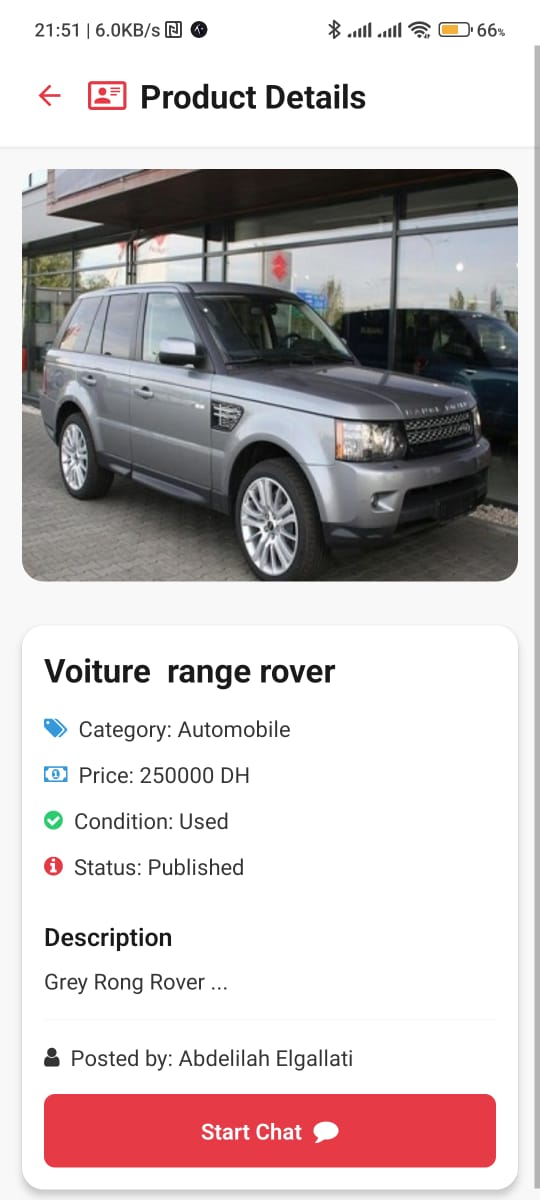
\includegraphics[width=0.8\textwidth]{images/product_details.png} % Remplacez par le chemin de votre capture d'écran
		\caption{Page de détails d'un produit. Cette interface affiche des informations détaillées sur le produit, y compris des photos, une description, le prix et les conditions d'échange.}
		\label{fig:product_details}
	\end{figure}
	
	\subsection{Messagerie intégrée}
	\begin{figure}[H]
		\centering
		\includegraphics[width=0.8\textwidth]{images/messaging.png} % Remplacez par le chemin de votre capture d'écran
		\caption{Messagerie intégrée. Les utilisateurs peuvent discuter et négocier les détails des transactions directement dans l'application.}
		\label{fig:messaging}
	\end{figure}
	
	\subsection{Tableau de bord utilisateur}
	\begin{figure}[H]
		\centering
		\includegraphics[width=0.8\textwidth]{images/user_dashboard.png} % Remplacez par le chemin de votre capture d'écran
		\caption{Tableau de bord utilisateur. Les utilisateurs peuvent suivre leurs transactions, gérer leurs produits et consulter leurs interactions.}
		\label{fig:user_dashboard}
	\end{figure}
	
	\section{Conclusion}
	Dans ce chapitre, nous avons détaillé les étapes de réalisation de notre application, en présentant les outils et technologies utilisés, le modèle de données, ainsi que l'architecture du système. La phase de mise en œuvre a permis de concrétiser notre vision théorique en une solution fonctionnelle. Grâce à une gestion rigoureuse des tâches et l'utilisation appropriée des technologies, nous avons surmonté les défis techniques pour répondre aux exigences du projet. Cette réussite témoigne de notre capacité à transformer des idées conceptuelles en solutions opérationnelles.
	
	
	\chapter*{Conclusion Générale}
	\newpage
	
	Ce projet vise à créer une application innovante pour faciliter l'échange de produits d'occasion de manière sécurisée et simplifiée. En intégrant des fonctionnalités variées telles que la gestion des utilisateurs, un catalogue organisé, une recherche avancée, ainsi que des systèmes de messagerie, de commentaires et d'évaluation, l'application répond aux besoins d'une communauté engagée dans la réutilisation des ressources. L'objectif principal est de promouvoir une culture de durabilité et de réduction du gaspillage, tout en assurant une expérience utilisateur fluide et efficace.
	
	À l'avenir, l'application peut évoluer en ajoutant de nouvelles fonctionnalités telles que des outils de traçabilité, des recommandations personnalisées et des systèmes de paiements sécurisés. De plus, une collaboration avec des organisations environnementales ou sociales pourrait enrichir l'application, en offrant des solutions innovantes pour une économie circulaire plus inclusive. En mettant l'accent sur la sécurité des utilisateurs et l'amélioration continue de l'expérience utilisateur, l'application restera pertinente et compétitive sur le marché du partage et de l'échange de produits d'occasion.
	
	Ce projet a non seulement renforcé nos compétences techniques et méthodologiques, mais il nous a également permis de comprendre les défis et les exigences du développement d'une application Mobile dans un contexte professionnel réel. Nous sommes convaincus que les compétences acquises durant ce projet seront des atouts précieux dans notre carrière future.
	
	\chapter*{Bibliographie et Références}
	\begin{itemize}
		\item \url{https://openclassrooms.com/fr/}
		\item \url{https://www.udemy.com/}
		\item \url{https://getbootstrap.com/}
		\item \url{https://www.dabadoc.com/ma}
		\item Chaine YouTube Bro Code : \url{https://youtu.be/zZ6vybT1HQs?si=I_gRa9sftSVMJQka}
		\item \url{https://www.canva.com/en_gb/}
	\end{itemize}

\end{document}